\subsubsection{UC 1 - \textit{Login}}
\begin{figure}[H]
    \vspace{2em}
    \centering
    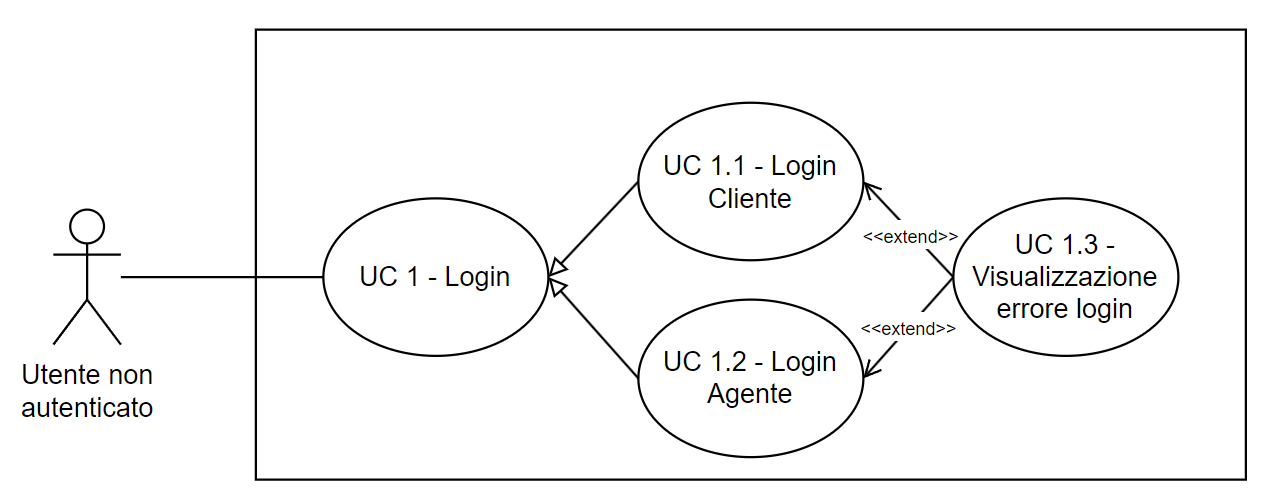
\includegraphics[width=0.75\columnwidth]{img/usecase/UC 1.png}
    \caption{\textit{Use Case} 1: \textit{Login} Utente}
    \label{fig:uc_1}
\end{figure}

\begin{usecase}{ 1}{\textit{Login} utente}
    \usecaseactors{Utente non autenticato.}
    \usecasedesc{L'utente ha inserito \textit{username} e \textit{password} per autenticarsi nell'\textit{app}.}
    \usecasepre{L'utente ha avviato l'\textit{app}.}
    \usecasepost{L'utente è autenticato nel sistema o ha ricevuto un errore.}
    \usecasescen{
        \begin{itemize}
            \item L'utente visualizza la schermata di \textit{login} di {\movi};
            \item L'utente inserisce lo \textit{username};
            \item L'utente inserisce la \textit{password};
            \item L'utente preme il pulsante per effettuare il \textit{login};
            \item L'utente viene autenticato ed entra nell'applicazione.
        \end{itemize}}
    \label{uc:uc_1}
\end{usecase}

\begin{usecase}{ 1.1}{\textit{Login} cliente}
    \usecaseactors{Utente non autenticato.}
    \usecasedesc{L'utente è un cliente dell'azienda e vuole autenticarsi nell'\textit{app}.}
    \usecasepre{L'utente ha avviato l'\textit{app}.}
    \usecasepost{L'utente è autenticato come cliente nel sistema o ha ricevuto un errore. Viene portato 
                 nella \texttt{Homepage} e nulla cambia rispetto la vecchia versione dell'\textit{app}.}
    \usecasescen{
        \begin{itemize}
            \item L'utente visualizza la schermata di \textit{login} di {\movi};
            \item L'utente inserisce lo \textit{username};
            \item L'utente inserisce la \textit{password};
            \item L'utente preme il pulsante per effettuare il \textit{login};
            \item L'utente viene autenticato e visualizza la \texttt{Homepage} dell'applicazione.
        \end{itemize}}
    \label{uc:uc_1.1}
\end{usecase}

\begin{usecase}{ 1.2}{\textit{Login} agente}
    \usecaseactors{Utente non autenticato.}
    \usecasedesc{L'utente è un agente dell'azienda e vuole autenticarsi nell'\textit{app}.}
    \usecasepre{L'utente ha avviato l'\textit{app}.}
    \usecasepost{L'utente è autenticato come agente nel sistema o ha ricevuto un errore. Viene portato 
                 nella \texttt{Homepage Agenti}.}
    \usecasescen{
        \begin{itemize}
            \item L'utente visualizza la schermata di \textit{login} di {\movi};
            \item L'utente inserisce lo \textit{username};
            \item L'utente inserisce la \textit{password};
            \item L'utente preme il pulsante per effettuare il \textit{login};
            \item L'utente viene autenticato e visualizza la \texttt{Homepage Agenti} dell'applicazione.
        \end{itemize}}
    \label{uc:uc_1.2}
\end{usecase}

\begin{usecase}{ 1.3}{Visualizzazione errore \textit{login}}
    \usecaseactors{Utente non autenticato.}
    \usecasedesc{L'utente vuole autenticarsi nell'\textit{app} ma ha inserito \textit{username} o \textit{password} non validi.}
    \usecasepre{L'utente ha avviato l'operazione di \textit{login}.}
    \usecasepost{L'utente visualizza un messaggio che lo avvisa del fallimento dell'operazione di \textit{login}.}
    \usecasescen{
        \begin{itemize}
            \item L'utente visualizza la schermata di \textit{login} di {\movi};
            \item L'utente inserisce lo \textit{username};
            \item L'utente inserisce la \textit{password};
            \item L'utente preme il pulsante per effettuare il \textit{login};
            \item L'utente visualizza un errore.
        \end{itemize}}
    \label{uc:uc_1.3}
\end{usecase}